\documentclass[smaller]{beamer}

\usepackage{helvet}
\usepackage{hyperref, graphicx}
\usepackage{amsthm}
\usepackage{amsfonts}
\usepackage{etoolbox}
\usepackage{wrapfig}
\usepackage{tikz}
\usetikzlibrary{backgrounds}
\usepackage{ulem}
\usepackage{fontspec}
%\usepackage[T1]{fontenc}
%\setmainfont{Cambria}
%\usefonttheme{serif}

\usetheme{default}
\setbeamertemplate{navigation symbols}{}
\AtBeginSection[ ]
{
\begin{frame}{Outline}
    \tableofcontents[currentsection]
\end{frame}
}

% Default fixed font does not support bold face
\DeclareFixedFont{\ttb}{T1}{txtt}{bx}{n}{11} % for bold
\DeclareFixedFont{\ttm}{T1}{txtt}{m}{n}{12}  % for normal - use in headings

% Custom colors
\usepackage{color}
\definecolor{TUGray}{RGB}{101,101,137}
\definecolor{TUBlack}{RGB}{30,0,0}
\definecolor{mygreen}{RGB}{45,111,63}
\definecolor{keywords}{RGB}{205,114,0}
\definecolor{comments}{RGB}{181,51,139}
\definecolor{strings}{RGB}{58,144,81}
\definecolor{numeric}{RGB}{66,110,176}
\definecolor{linos}{rgb}{0.4,0.4,0.4}
\definecolor{links}{rgb}{0,0.4,0.75}

\definecolor{bggray}{RGB}{232, 233, 235}

\definecolor{cerulean}{RGB}{4, 133, 209}

\usecolortheme[named=mygreen]{structure}
\setbeamercolor{normal text}{fg=TUBlack}\usebeamercolor*{normal text}

\setbeamercolor{codecol}{fg=TUGray!25!black,bg=bggray}

\hypersetup{colorlinks, linkcolor=links, urlcolor=links}



\usepackage[sfdefault,scaled=.85]{FiraSans}
\usepackage{newtxsf}

\usepackage{listings}

\newtoggle{InString}{}% Keep track of if we are within a string
\togglefalse{InString}% Assume not initally in string

\newcommand\digitstyle{\color{numeric}}
\makeatletter
\newcommand{\ProcessDigit}[1]
{%
  \ifnum\lst@mode=\lst@Pmode\relax%
   {\digitstyle #1}%
  \else
    #1%
  \fi
}
\makeatother

\lstset{literate=%
    {0}{{{\ProcessDigit{0}}}}1
    {1}{{{\ProcessDigit{1}}}}1
    {2}{{{\ProcessDigit{2}}}}1
    {3}{{{\ProcessDigit{3}}}}1
    {4}{{{\ProcessDigit{4}}}}1
    {5}{{{\ProcessDigit{5}}}}1
    {6}{{{\ProcessDigit{6}}}}1
    {7}{{{\ProcessDigit{7}}}}1
    {8}{{{\ProcessDigit{8}}}}1
    {9}{{{\ProcessDigit{9}}}}1
	{<=}{{\(\leq\)}}1
	{>=}{{\(\geq\)}}1,
	% morestring=[b]",
    % morestring=[b]',
    % morecomment=[l]{//},
}

\lstdefinelanguage{Pseudo}{
    morekeywords={return, while, if, for, input},
    morecomment=[l]{\#},
}

% Pseudocode style
\newcommand\pseudostyle{\lstset{
language=Pseudo,
basicstyle=\fontfamily{ccr}\scriptsize,
commentstyle=\it\scriptsize\color{linos},
keywordstyle=\it\bfseries\scriptsize,
mathescape=true,
literate=
    {=}{$\leftarrow{}$}{1}
    {==}{$={}$}{1}
    {<=}{{\(\leq\)}}1
	{>=}{{\(\geq\)}}1,
xleftmargin=18pt,
xrightmargin=4pt,
aboveskip=12pt,
belowskip=0pt,
frame=tB,
keepspaces=true
}}

% Python style for highlighting
\newcommand\pythonstyle{\lstset{
language=Python,
basicstyle=\ttfamily\tiny,
numbers=left,
numberstyle=\tiny\color{linos},
morekeywords={self, np},              % Add keywords here
keywordstyle=\tiny\color{keywords},
commentstyle=\it\tiny\color{comments},    % Custom highlighting style
stringstyle=\tiny\color{strings},
xleftmargin=18pt,
xrightmargin=4pt,
aboveskip=0pt,
belowskip=0pt,
escapeinside={(*@}{@*)},
frame=l,                         % Any extra options here
showstringspaces=false,
keepspaces=true
}}

% Pseudocode environment
\lstnewenvironment{pseudo}[1][]
{
    \pseudostyle
    \lstset{
        #1
    }
}
{}

% Python environment 
\lstnewenvironment{python}[1][]
{
	\pythonstyle
	\lstset{
	#1
	}
}
{}

% wrap the Python environment
\newenvironment{codeblock}
    {\hfill\begin{beamerboxesrounded}[lower=codecol, width=0.8\textwidth]
    \medskip

    }
    { 
    \end{beamerboxesrounded}\hfill
    }

\theoremstyle{example}
\newtheorem{question}{Question}

\newcommand{\ct}[1]{\lstinline[language=Python]!#1!}
\newcommand{\ttt}[1]{{\small\texttt{#1}}}
\newcommand{\lsitem}[2]{\ttt{{#1}[}\ct{#2}\ttt{]}}

\newcommand{\x}{\textbf{x}}
\newcommand{\ix}[1]{{\it #1}}

\author{Chris Cornwell}
\date{April 29, 2025}
\title{Distance in High Dimensions and Clustering}

\begin{document}

\begin{frame}
\titlepage
\end{frame}

\begin{frame}
    \frametitle{Outline}
    \tableofcontents
\end{frame}

\section{The Curse of Dimensionality}

%%%%
\begin{frame}
    \frametitle{Clustering uses Distance}

    \begin{minipage}{\textwidth}
    \begin{wrapfigure}{r}{0.4\textwidth}
        \begin{center}
            %\vspace{-\baselineskip}
            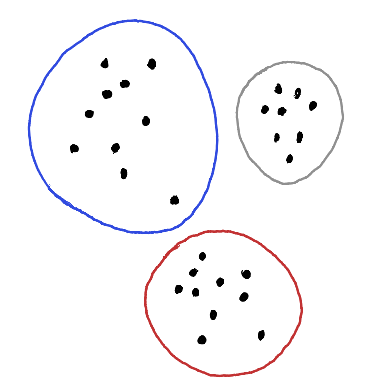
\includegraphics[height=0.4\textheight]{../../Images/clusters.png}
        \end{center}
    \end{wrapfigure}

    \vspace{\baselineskip}
    \mbox{Aim of clustering:} group the training data $\mathcal S$ into \textbf{clusters} $C_1,C_2,\ldots,C_k$, with every point in some cluster $C_i$ (i.e., $\mathcal S=C_1\cup C_2\cup\ldots \cup C_k$) and clusters are disjoint.\footnote{These conditions are the common ones. However, sometimes one may wish to exclude an \textit{outlier} from being in a cluster, and sometimes clusters are ``fuzzy,'' meaning that points have a probability for being in each cluster.} 
    
    \pause
    \vspace{8pt}
    Goal:
    have points in the same cluster to be ``similar''.

    \pause
    \vspace{8pt}
    While most types of ML algorithms are affected by how densely points are packed in $\mathcal S$, clustering algorithms typically use distance (to the nearest points in $\mathcal S$) to measure similarity of points. 
    \end{minipage}

    \pause
    \begin{itemize}
        \item Makes a phenomenon called the \textbf{curse of dimensionality} especially relevant.
    \end{itemize}  

\end{frame}

%%%%
\begin{frame}
    \frametitle{What is the Curse of Dimensionality?}
    Not universally, clearly defined what falls under the umbrella of the curse of dimensionality and what does not. 
    \pause
    \begin{itemize}
        \item Strict interpretation: The amount of training data used needs to increase exponentially in the number of features, i.e., independent variables. (If the number of samples needed to see how position/value of one feature might affect $\ix y$ labeling is roughly constant over the features.)
        \pause
        \item Broad interpretation: With large number of features (so, large $d$, where $\x_i\in\mathbb R^d$), our intuition for the way that the distance between points relates to properties we care about will break down.\newline 
        Distance in high dimensions is \textit{weird}. (\textit{Let's see how}.)
    \end{itemize}
\end{frame}

%%%%
\begin{frame}
    \frametitle{Spheres in $\mathbb R^d$, $d$ large: weird}
    Often, work with those points that are within a given distance $R$ from fixed point. These are points in a $d$-dimensional ``ball'' (that is, enclosed by a $d$-dimensional sphere): 
            \[B_R(\textbf{p}) = \{\x\in\mathbb R^d\ |\ |\x - \textbf{p}| \le R\}.\]
    \pause
    (\textit{Distance} here is $|\x - \textbf{p}| = \sqrt{\sum_{i=1}^d(x_i-p_i)^2}$, usual Euclidean norm.)

    \pause
    \vspace{\baselineskip}
    The volume of $B_R(\textbf{p})$: \qquad $\frac{\pi^{d/2}}{\Gamma(\frac{d}{2} + 1)}R^d$.

    \vspace{\baselineskip}
    $\Gamma$ is Euler's gamma function. If $d$ is even, $\Gamma(\frac{d}{2}+1) = (\frac{d}{2})!$ and if $d$ is odd, it's roughly similar: $(\frac{d}{2})(\frac{d}{2}-1)\ldots(\frac12)\pi^{1/2}$.

    \pause
    \centering
    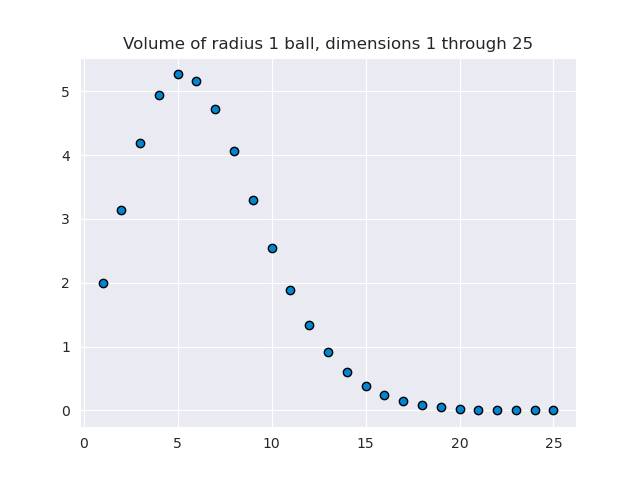
\includegraphics[height = 0.3\textheight]{../../Images/UnitBallVolume.png}

\end{frame}

%%%%
\begin{frame}
    \frametitle{Most points are near boundary}
    So, for any fixed radius $R>0$, the volume of the $d$-dimensional $B_R(\textbf{p})$ approaches $0$ as $d\to\infty$.  

    \pause
    Additionally, \textit{where} the space/volume within $B_R(\textbf{p})$ is distributed changes as dimension increases. 

    \pause
    Choose $\varepsilon$ with $0 < \varepsilon < R$. What proportion of points in $B_R(\textbf{p})$ are at least $\varepsilon$ away from the boundary sphere? That is, how large is $B_{R-\varepsilon}(\textbf{p})$ in comparison to $B_{R}(\textbf{p})$? \pause \ In dimension $d=2$, with $R=1$:

    \[\frac{\operatorname{Vol}B_{1-\varepsilon}}{\operatorname{Vol}B_{1}} = 
    \frac{\pi(1-\varepsilon)^2}{\pi} = (1-\varepsilon)^2.
    \]
    \pause
    For example, if $\varepsilon =0.05$ then this is a little more than $0.9$.

    \pause
    Generally, 
    \[\frac{\operatorname{Vol}B_{R-\varepsilon}}{\operatorname{Vol}B_{R}} = 
    \frac{\pi^{d/2}(R-\varepsilon)^d}{\Gamma(d/2 + 1)}\frac{\Gamma(d/2+1)}{\pi^{d/2}R^d} = \left(\frac{R-\varepsilon}{R}\right)^d = \left(1 - \frac{\varepsilon}{R}\right)^d.
    \]
    Since $1-\frac{\varepsilon}{R} < 1$, this approaches $0$ as $d\to\infty$.\pause\  Returning to $\varepsilon=0.05$ and $R=1$, the ratio is less than $0.05$ if $d \ge 59$; so, more than 95\% of the volume of $B_{R}(\textbf{p})$ is contained in an outer shell, within 0.05 of the boundary.
\end{frame}

%%%%
\begin{frame}
    \frametitle{Most points are near boundary}
    A consequence? 
    
    \begin{itemize}
        \item Given a point, say you randomly select some points in data from those that are within a given distance of it. \newline 
        \pause
        The higher the dimension, the more likely these points will be nearly equal distance from the chosen point. So, which \textit{one} is closest is more subject to random chance (from a small amount of noise, say). 
    \end{itemize}

    \pause
    Increasingly likely, also, that none of these points are near each other:\pause \ points below sampled with random coordinates (i.i.d., with a mean-zero normal distribution). Distances between all pairs of sampled points were calculated and plotted in a histogram. 

    \centering
    \begin{figure}
        \begin{minipage}{0.32\textwidth}
            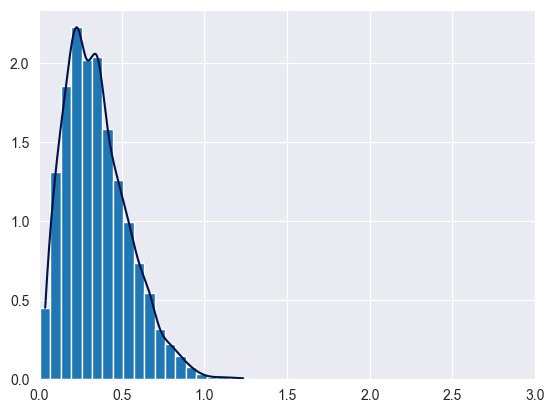
\includegraphics[width=\textwidth]{../../Images/pairwise-distances-dim2.png}
        \end{minipage}
        \hfill
        \begin{minipage}{0.32\textwidth}
            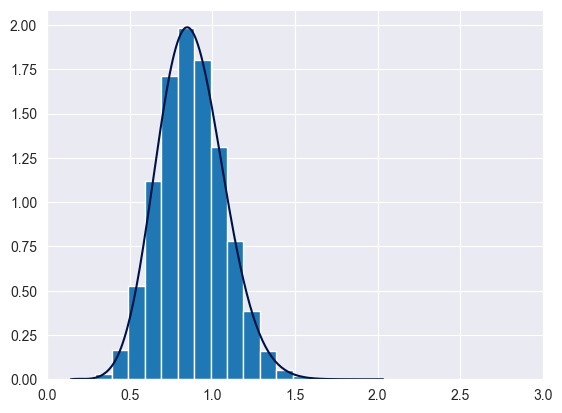
\includegraphics[width=\textwidth]{../../Images/pairwise-distances-dim10.png}
        \end{minipage}
        \hfill
        \begin{minipage}{0.32\textwidth}
            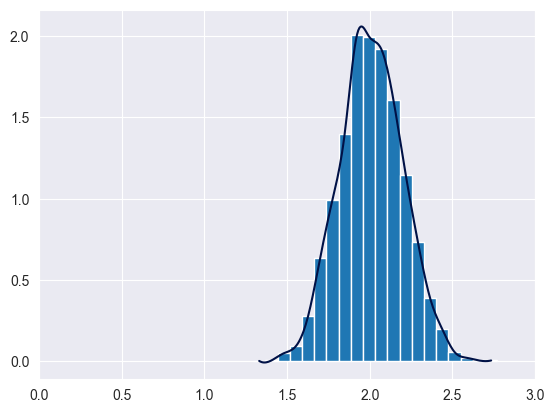
\includegraphics[width=\textwidth]{../../Images/pairwise-distances-dim50.png}
        \end{minipage}
        \caption{Left: points in $\mathbb R^2$; Middle: points in $\mathbb R^{10}$; Right: points in $\mathbb R^{50}$}
    \end{figure}
\end{frame}

%%%%
\begin{frame}
    \frametitle{Another example of high dimensional weirdness}
    \begin{minipage}{\textwidth}
    \begin{wrapfigure}{r}{0.35\textwidth}
        \begin{center}
            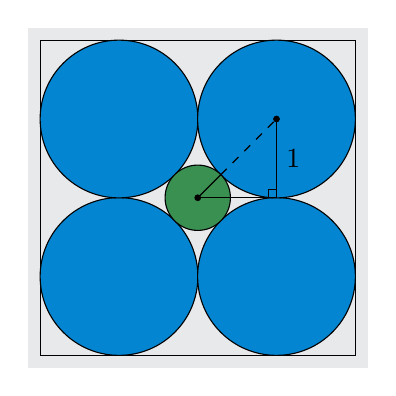
\begin{tikzpicture}[background rectangle/.style={fill=bggray}, show background rectangle]
                \draw[black] (0,0) -- (4,0) -- (4,4) -- (0,4) -- cycle;
                \foreach \x in {1,3}
                    \foreach \y in {1,3}
                        \filldraw[fill=cerulean] (\x,\y) circle (28.5pt);
                \filldraw[fill=strings] (2,2) circle (11.803pt);
                \foreach \x in {2,3}
                    \filldraw[fill=black] (\x,\x) circle (1pt);
                \draw[black] (2,2) -- (3,2) --node[right]{$1$} (3,3);
                \draw[black] (2.9,2) -- (2.9,2.1) -- (3,2.1);
                \draw[black] (2,2) -- (2+0.4142/1.4142, 2+0.4142/1.4142);
                \draw[black, dashed] (2+0.4142/1.4142, 2+0.4142/1.4142) -- (3,3);
            \end{tikzpicture}
        \end{center}
        \caption{Filling 2D square with corner circles and center circle}
    \end{wrapfigure}

    In $\mathbb R^2$, consider the five depicted circles in the square $[-2,2]^2$. The four ``corner'' circles are tangent to (two) edges of the square and tangent to each other. Each of them has radius 1. The ``center'' circle has center at the origin and is tangent to all four corner circles.

    \pause
    The radius of the center circle is $\sqrt{2} - 1\approx 0.414$. Hence, it is smaller than each of the corner circles (as is visibly apparent).

    \pause
    Generalize this: the (hyper)cube $[-2,2]^d$ in $\mathbb R^d$. In general, there are $2^d$ corner spheres, each with radius 1. There is one center sphere, with the origin as its center (same as the hypercube) and which is tangent to all corner spheres.
    \end{minipage}
\end{frame}

%%%%
\begin{frame}
    \frametitle{Another example of high dimensional weirdness}
    As a consequence of the distance formula in $\mathbb R^d$, the radius of the center sphere is necessarily $\sqrt{d} - 1$.\pause \ Note the consequences: 
    \begin{itemize}
        \item When $d=4$, then the center sphere is the same size as the corner spheres, since $\sqrt{4}-1 = 1$.
        \pause
        \item The center sphere is larger than the corner spheres when $d\ge 5$, and once $d = 9$ we have that the radius of the center sphere is $2$. So, that center sphere intersects the boundary of the cube.
        \pause
        \item For $d\ge 10$, the center sphere contains points that are \textit{outside of} the hypercube. (Despite still being tangent to all $2^d$ corner spheres, which ``surround'' it and are \textit{entirely contained} within the hypercube.
    \end{itemize}
\end{frame}

\section{Clustering Methods}

\begin{frame}
    \frametitle{$k$-means Clustering}
    We previously spent time on $k$-means clustering. Here is a quick recap for data $\mathcal S = \{(\x_i, \ix y_i)\}_{i=1}^n$, with $\x_i\in\mathbb R^d$.
    
    \onslide<2->{
    You choose $k$, the number of clusters and randomly initialize $k$ centroids $\mu_1,\mu_2,\ldots \mu_k$, each $\mu_i\in\mathbb R^d$. Clusters $C_1,C_2,\ldots, C_k$ are determined as follows. }

    \begin{enumerate}
        \onslide<3->{
        \item For each data point $\x_i$, determine $j(i)$ with $1\le j(i)\le k$, so that $\mu_{j(i)}$ is the closest centroid to $\x_i$. Then, $\x_i \in C_j$ precisely when $j=j(i)$. }
        \onslide<4->{
        \item Update $\mu_1,\mu_2,\ldots,\mu_k$ so that, for $1\le j\le k$, the centroid of $C_j$ is $\mu_j$, i.e., $\mu_j = \frac{1}{|C_j|}\sum_{\x_i\in C_j}\x_i$. }
        \onslide<5->{
        \item Iterate steps {\color{mygreen}1} and {\color{mygreen}2} until the assignment $i\mapsto j(i)$ that is made in {\color{mygreen}1} is the same as it was in the previous iteration. }
    \end{enumerate}

    \vspace*{-6pt}
    \begin{figure}
            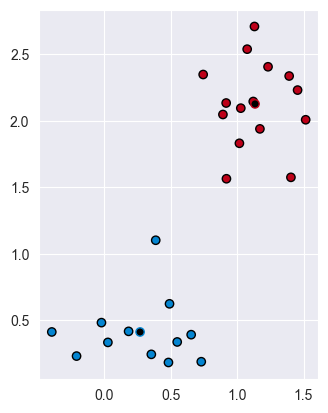
\includegraphics[height=0.3\textheight]{../../Images/kmeans_4.png}
        \caption{Result of $k$-means, 2 centroids in black}
    \end{figure}
\end{frame}

%%%%
\begin{frame}
    \frametitle{$k$-means Clustering}
    \begin{enumerate}
        \item For each data point $\x_i$, determine $j(i)$ with $1\le j(i)\le k$, so that $\mu_{j(i)}$ is the closest centroid to $\x_i$. Then, $\x_i \in C_j$ precisely when $j=j(i)$.
        \item Update $\mu_1,\mu_2,\ldots,\mu_k$ so that, for $1\le j\le k$, the centroid of $C_j$ is $\mu_j$, i.e., $\mu_j = \frac{1}{|C_j|}\sum_{\x_i\in C_j}\x_i$.
        \item Iterate steps {\color{mygreen}1} and {\color{mygreen}2} until the assignment $i\mapsto j(i)$ that is made in {\color{mygreen}1} is the same as it was in the previous iteration.
    \end{enumerate}
    \vfill

    \begin{minipage}{\textwidth}
    \begin{wrapfigure}{r}{0.3\textwidth}
            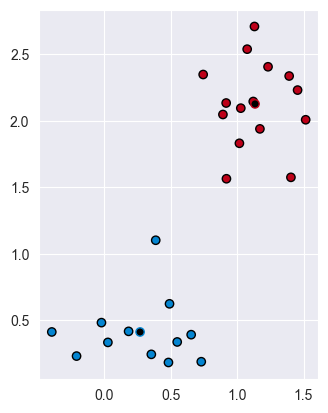
\includegraphics[height=0.3\textheight]{../../Images/kmeans_4.png}
        \caption{Result of $k$-means, 2 centroids in black}
    \end{wrapfigure}

    In any iteration of {\color{mygreen}1}, for $\x_i$ to change its cluster, it is necessary that $|\x_i - \mu_{j(i)}|$ decreases, so \mbox{$\sum_{i=1}^n|\x_i - \mu_{j(i)}|^2$} decreases.\pause \ In any iteration of {\color{mygreen}2}, setting $\mu_j = \frac{1}{|C_j|}\sum_{\x_i\in C_j}\x_i$ will minimize $\sum_{\x_i\in C_j}|\x_i-\mu_j|^2$, and so $\sum_{i=1}^n|\x_i - \mu_{j(i)}|^2$ decreases (or stays the same) on this step.

    \pause
    Thus, the algorithm terminates: there are finitely many points in $\mathcal S$, so there are only a finite number of possibilities for the list $\mu_1, \mu_2, \ldots, \mu_k$.
    \end{minipage}
\end{frame}

\begin{frame}[fragile]
    \frametitle{DBSCAN Clustering}
    DBSCAN (Density-Based Spatial Clustering for Applications with Noise) does not require you to choose a number of clusters at the start.
    
    \pause 
    There are two important hyperparameters that you choose: 
    \begin{itemize}
        \item $\varepsilon$ (\ttt{eps} in scikit-learn, a certain radius in the procedure); and 
        \pause
        \item \ttt{minPts} (\lstinline[language=Python,basicstyle=\ttfamily]{min_samples} in scikit-learn).
    \end{itemize}

    \begin{minipage}{\textwidth}
    \begin{wrapfigure}{r}{0.35\textwidth}
        \vspace{-\baselineskip}
        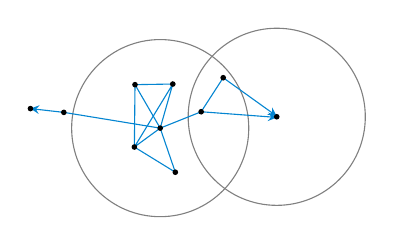
\begin{tikzpicture}[>=stealth,scale=0.8]
            \draw[gray] (0,0) circle (40pt);
            \draw[gray] (1.85,0.18) circle (40pt);
            \draw[cerulean] (0,0) -- (0.2,0.7) -- (-0.4,0.69) -- (-0.41,-0.3) -- (0,0) -- (0.24,-0.7) -- (-0.41,-0.3) -- (0.2,0.7);
            \draw[cerulean] (0,0) -- (-0.4,0.69);
            \draw[cerulean] (0,0) -- (-1.53,0.25);
            \draw[cerulean, ->] (-1.53,0.25) -- (-2.06,0.31);
            \draw[cerulean] (0,0) -- (0.65,0.26) -- (1,0.8); 
            \draw[cerulean, ->] (1,0.8) -- (1.85,0.19);
            \draw[cerulean, ->] (0.65,0.26) -- (1.85,0.17);
            \foreach \p in {(0,0), (0.2,0.7), (0.24,-0.7), (-0.4,0.69), (-0.41,-0.3), (0.65,0.26), (1,0.8), (1.85,0.18), (-1.53,0.25), (-2.06,0.31)}
                \filldraw \p circle (1pt);
        \end{tikzpicture}
        \caption{Points reachable from core point, \ttt{minPts}$=4$}
    \end{wrapfigure}

    \pause
    \vspace{\baselineskip}
    Describing how clusters are formed requires some terminology. 
    
    \pause
    As with $k$-means, the distance function (metric) that is used is a central part of the process. Unlike the centroids used in $k$-means, though, a different metric would not require a change to the procedure (other than different distance computations). 
    \end{minipage}
\end{frame}

\begin{frame}
    \frametitle{DBSCAN Clustering}
    Have (training) data $\mathcal S \subset\mathbb R^d$ (no label given for an $\x\in\mathcal S$). Write $d(\textbf{p}, \textbf{q})$ for the distance between points $\textbf{p}$ and $\textbf{q}$, which could be distance in any metric.
    \pause
    \begin{itemize}
        \item Any $\textbf{p}\in\mathcal S$ is a \textbf{core point} if \ttt{minPts} training samples are within $\varepsilon$ of it; so,
            \[\#\{\x\in\mathcal S\ |\ d(\textbf{p}, \x) < \varepsilon\} \ge \ttt{minPts}.\]
        \item  \pause Given core point $\textbf{p}$, and $\x \in \mathcal S$, $\x$ is \textbf{directly reachable} from $\textbf{p}$ if $d(\textbf{p}, \x) < \varepsilon$. 
        \pause
        \item Given core point $\textbf{p}$, and $\x \in \mathcal S$, $\x$ is \textbf{reachable} from $\textbf{p}$ if there exist $\textbf{p}_1, \ldots, \textbf{p}_m$ such that $\textbf{p}_{i+1}$ is directly reachable from $\textbf{p}_i$, all $1\le i \le m-1$, and $\textbf{p}_1=\textbf{p}$, $\textbf{p}_m=\x$.
    \end{itemize}
    
    
    \begin{minipage}{\textwidth}
        \begin{wrapfigure}{r}{0.35\textwidth}
            \vspace{-2\baselineskip}
            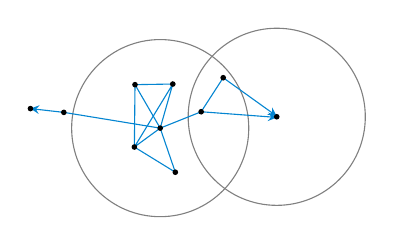
\begin{tikzpicture}[>=stealth,scale=0.8]
                \draw[gray] (0,0) circle (40pt);
                \draw[gray] (1.85,0.18) circle (40pt);
                \draw[cerulean] (0,0) -- (0.2,0.7) -- (-0.4,0.69) -- (-0.41,-0.3) -- (0,0) -- (0.24,-0.7) -- (-0.41,-0.3) -- (0.2,0.7);
                \draw[cerulean] (0,0) -- (-0.4,0.69);
                \draw[cerulean] (0,0) -- (-1.53,0.25);
                \draw[cerulean, ->] (-1.53,0.25) -- (-2.06,0.31);
                \draw[cerulean] (0,0) -- (0.65,0.26) -- (1,0.8); 
                \draw[cerulean, ->] (1,0.8) -- (1.85,0.19);
                \draw[cerulean, ->] (0.65,0.26) -- (1.85,0.17);
                \foreach \p in {(0,0), (0.2,0.7), (0.24,-0.7), (-0.4,0.69), (-0.41,-0.3), (0.65,0.26), (1,0.8), (1.85,0.18), (-1.53,0.25), (-2.06,0.31)}
                    \filldraw \p circle (1pt);
            \end{tikzpicture}
            \caption{Points reachable from core point, \ttt{minPts}$=4$}
        \end{wrapfigure}
    
    \pause
    \vspace{\baselineskip}
    With this terminology, let $\textbf{p}\in\mathcal S$ be a core point. The cluster, $C_{\textbf{p}}$ say, is the set of all points in $\mathcal S$ (including $\textbf{p}$) that are reachable from $\textbf{p}$.\pause \ A point in $C_{\textbf{p}}$ that is not a core point might be considered the ``edge'' of the cluster, as no point may be reached from it.
    \end{minipage}
\end{frame}

\end{document}